\documentclass[tikz,border=10pt]{standalone}
\usepackage{amsmath, amssymb, bm}
\usetikzlibrary{positioning, arrows.meta, calc, fit, backgrounds}

\begin{document}
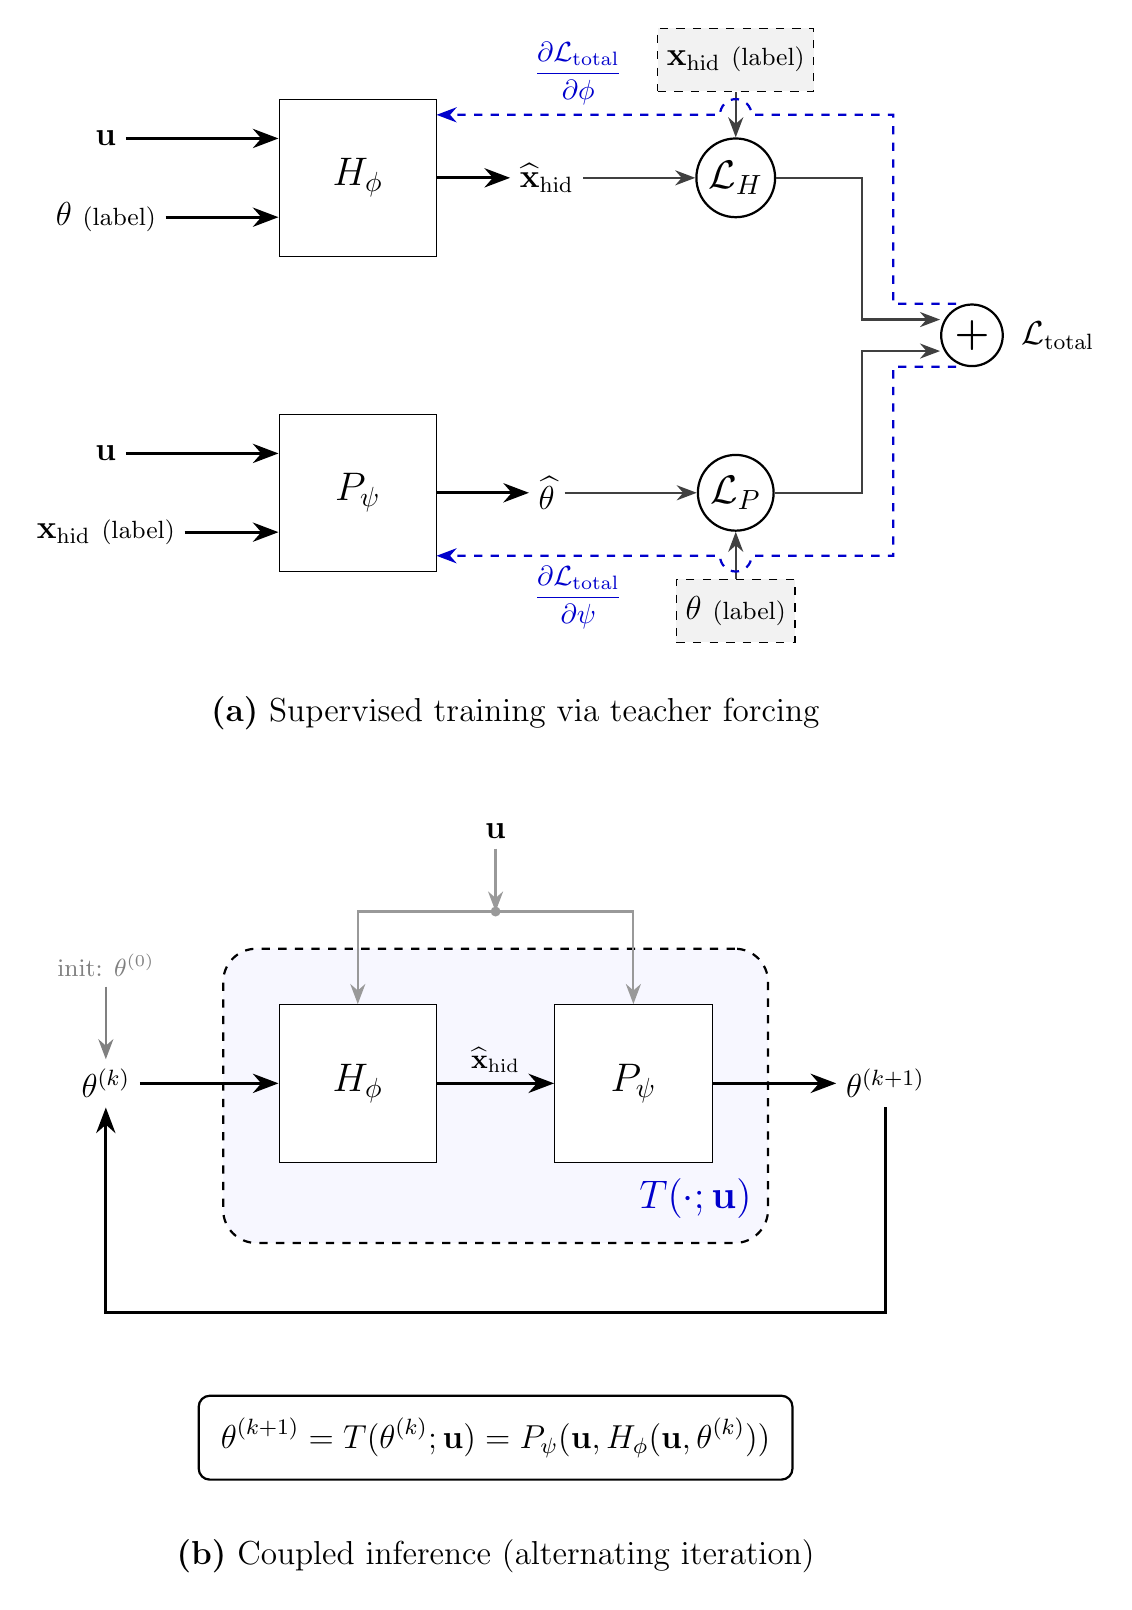
\begin{tikzpicture}[
    >={Stealth[scale=1.1]},
    netbox/.style={draw, rectangle, minimum width=2.0cm, minimum height=2.0cm, align=center, font=\Large, fill=white},
    txt/.style={align=center, font=\large},
    eqbox/.style={draw, rectangle, rounded corners, inner sep=8pt, font=\large, thick},
    labelbox/.style={draw, dashed, rectangle, minimum width=1.5cm, minimum height=0.8cm, align=center, fill=gray!10, font=\large},
    lossnode/.style={draw, circle, inner sep=2pt, font=\Large, thick},
    uarrow/.style={->, thick, gray!80},
    mainarrow/.style={->, very thick, black},
    dataarrow/.style={->, thick, darkgray},
    backproparrow/.style={->, thick, dashed, blue!80!black}
]

% ==========================================
% PANEL (a) : Training (Teacher Forcing)
% ==========================================
\begin{scope}
    % H_phi Block & Inputs
    \node[netbox] (H_train) at (0, 0) {$H_\phi$};
    \node[txt] (u_H) at (-3.2, 0.5) {$\mathbf{u}$};
    \node[txt] (theta_H) at (-3.2, -0.5) {$\theta$ \small{(label)}};
    \draw[mainarrow] (u_H.east) -- (H_train.west |- u_H.east);
    \draw[mainarrow] (theta_H.east) -- (H_train.west |- theta_H.east);

    % H_phi Output & Loss
    \node[txt] (xhat_H) at (2.4, 0) {$\widehat{\mathbf{x}}_{\mathrm{hid}}$};
    \draw[mainarrow] (H_train.east) -- (xhat_H.west);
    \node[lossnode] (LossH) at (4.8, 0) {$\mathcal{L}_H$};
    \node[labelbox] (target_H) at (4.8, 1.5) {$\mathbf{x}_{\mathrm{hid}}$ \small{(label)}};
    \draw[dataarrow] (xhat_H.east) -- (LossH.west);
    \draw[dataarrow] (target_H.south) -- (LossH.north);

    % P_psi Block & Inputs
    \node[netbox] (P_train) at (0, -4.0) {$P_\psi$};
    \node[txt] (u_P) at (-3.2, -3.5) {$\mathbf{u}$};
    \node[txt] (xhid_P) at (-3.2, -4.5) {$\mathbf{x}_{\mathrm{hid}}$ \small{(label)}};
    \draw[mainarrow] (u_P.east) -- (P_train.west |- u_P.east);
    \draw[mainarrow] (xhid_P.east) -- (P_train.west |- xhid_P.east);

    % P_psi Output & Loss
    \node[txt] (thetahat_P) at (2.4, -4.0) {$\widehat{\theta}$};
    \draw[mainarrow] (P_train.east) -- (thetahat_P.west);
    \node[lossnode] (LossP) at (4.8, -4.0) {$\mathcal{L}_P$};
    \node[labelbox] (target_P) at (4.8, -5.5) {$\theta$ \small{(label)}};
    \draw[dataarrow] (thetahat_P.east) -- (LossP.west);
    \draw[dataarrow] (target_P.north) -- (LossP.south);

    % Total Loss
    \node[draw, circle, inner sep=2pt, font=\Large, thick] (Sum) at (7.8, -2.0) {$\bm{+}$};
    \node[txt, right=0.1cm of Sum] (L_total) {$\mathcal{L}_{\text{total}}$};
    \draw[dataarrow] (LossH.east) -| (6.4, -1.8) -- (Sum.west |- 0,-1.8);
    \draw[dataarrow] (LossP.east) -| (6.4, -2.2) -- (Sum.west |- 0,-2.2);

    % Backpropagation
    \draw[backproparrow] (7.6, -1.6) -| (6.8, 0.8) -- (5.0, 0.8) arc[start angle=0, end angle=180, radius=0.2cm] -- node[midway, above] {$\displaystyle \frac{\partial \mathcal{L}_{\mathrm{total}}}{\partial \phi}$} (1.0, 0.8);
    \draw[backproparrow] (7.6, -2.4) -| (6.8, -4.8) -- (5.0, -4.8) arc[start angle=0, end angle=-180, radius=0.2cm] -- node[midway, below] {$\displaystyle \frac{\partial \mathcal{L}_{\mathrm{total}}}{\partial \psi}$} (1.0, -4.8);

    % Subcaption for Panel (a) (하단 중앙 배치)
    \node[font=\large, align=center] at (2.0, -6.8) {\textbf{(a)} Supervised training via teacher forcing};
\end{scope}

% ==========================================
% PANEL (b) : Inference (Alternating)
% ==========================================
% 상하 간격을 적절히 유지하기 위해 yshift를 -12.5cm로 설정
\begin{scope}[yshift=-11.5cm] 
    % Network Blocks
    \node[netbox] (H_inf) at (0,0) {$H_\phi$};
    \node[netbox] (P_inf) at (3.5,0) {$P_\psi$};

    % T Operator Box
    \begin{scope}[on background layer]
        \node (dummy_bottom) at (3.5, -1.2) {}; 
        \node[draw, rounded corners=12pt, dashed, thick, inner sep=20pt, fit=(H_inf) (P_inf) (dummy_bottom), fill=blue!3] (Tbox) {};
        \node[font=\Large\bfseries, text=blue!80!black, anchor=south east, xshift=-0.1cm, yshift=0.2cm] at (Tbox.south east) {$T(\cdot; \mathbf{u})$};
    \end{scope}

    % Dynamic Variables
    \node[txt] (theta_in) at (-3.2, 0) {$\theta^{(k)}$};
    \node[txt, font=\small, text=gray] (init) at (-3.2, 1.5) {init: $\theta^{(0)}$};
    \node[txt] (theta_out) at (6.7, 0) {$\theta^{(k+1)}$};

    % Global Parameter (u)
    \node[txt] (u_input) at (1.75, 3.2) {$\mathbf{u}$};
    \draw[uarrow] (u_input.south) -- ++(0,-0.8) coordinate (u_split);
    \draw[uarrow] (u_split) -| (H_inf.north);
    \draw[uarrow] (u_split) -| (P_inf.north);
    \fill[gray!80] (u_split) circle (1.8pt);

    % Main Flow
    \draw[->, gray, thick] (init) -- (theta_in);
    \draw[mainarrow] (theta_in) -- (H_inf.west);
    \draw[mainarrow] (H_inf.east) -- (P_inf.west) node[midway, above] {$\widehat{\mathbf{x}}_{\mathrm{hid}}$};
    \draw[mainarrow] (P_inf.east) -- (theta_out.west);

    % Feedback Loop
    \draw[mainarrow] (theta_out.south) -- ++(0,-2.6) coordinate (loop_right) -- (loop_right -| theta_in.south) coordinate (loop_left) -- (theta_in.south);

    % Equation Box
    \node[eqbox] (eq) at (1.75, -4.5) {
        $\displaystyle \theta^{(k+1)} = T(\theta^{(k)}; \mathbf{u}) = P_\psi(\mathbf{u}, H_\phi(\mathbf{u}, \theta^{(k)}))$
    };

    % Subcaption for Panel (b) (하단 중앙 배치)
    \node[font=\large, align=center] at (1.75, -6.0) {\textbf{(b)} Coupled inference (alternating iteration)};
\end{scope}

\end{tikzpicture}
\end{document}